\documentclass[10pt, a4paper, twoside, openright]{report}

\usepackage[brazil]{babel}
\usepackage{url}
\usepackage{amssymb,amsxtra} %amsthm, amsxtra,dsfont}%}%
\usepackage[dvips=false, pdftex=false, vtex=false]{geometry}

\geometry{
 dvips=true, dvipdfm=true, pdftex=true, verbose, twoside, a4paper,
 headsep=1.00cm, footskip=1.00cm,
 %headheight=1.25em,
 paperwidth = 16.00truecm, paperheight = 23.00truecm,
 footnotesep=0.5cm,
 includehead, includefoot, ignoremp,
 hdivide = {2.00truecm,12.7truecm ,1.30truecm},  vdivide = {1.3truecm, ,1.30truecm}
}

%\usepackage[a4,center,font=textsf,frame]{crop}  %frame ou cam
\usepackage[a4,center,font=textsf,cam]{crop}
\setcounter{tocdepth}{4}
\setcounter{secnumdepth}{3}

\usepackage{makeidx}%showidx
\usepackage{graphicx,color}
\usepackage{fancyhdr}

\pagestyle{fancy}
\renewcommand{\chaptermark}[1]{\markboth{Cap.$\, $\thechapter \hspace{1em} #1}{}}
%% ==============================
\fancyhead{}% clear all fields\rhead{\nouppercase{\leftmark}}
%\fancyhead[LO]{\scriptsize\nouppercase{\sc\rightmark}}%
\fancyhead[LO]{}
\fancyhead[CO]{\scriptsize\nouppercase{\sc\rightmark}}%
%\fancyhead[RO]{~\mbox{\thepage}\hspace{-1.5em}}%
\fancyhead[RO]{~\mbox{\thepage}\hspace{0.0em}}%
%\fancyhead[RE]{\scriptsize\rm\nouppercase{\sc\leftmark}}%
%\fancyhead[LE]{\hspace{-1.5em}\mbox{\bf\textcolor[gray]{.60}\thepage}~}%
\fancyhead[LE]{\thepage}
\fancyhead[RE]{\footnotesize\rm\nouppercase{\sc  Cap\'{\i}tulo~\thechapter}}
\fancyfoot{}
%\fancyfoot[LO]{}%{2004}
%\fancyfoot[RE]{{\scriptsize 2009}}
%\fancyfoot[LE]{{\scriptsize\sc ed. ACMO}}
%\fancyfoot[RO]{}
%\fancyfoot[CE]{}%\textsc{\scriptsize\textmd{T\'{o}picos Breves de Matem\'{a}tica}}}
%\fancyfoot[CO]{\textsc{\scriptsize\textmd{QCD Perturbativa}}}
%
\renewcommand{\headrulewidth}{0.025pt}%{0.1pt}
\renewcommand{\footrulewidth}{0.0pt}%{0.1pt}

\usepackage[nottoc]{tocbibind}% coloca refer\^{e}ncia e \'{\i}ndice no sum\'{a}rio.
\usepackage[font=small,labelfont=bf,indention=1.5em]{caption}% <<===== CAPTION
\captionsetup[table]{position=top}%{position=top}
\captionsetup[figure]{position=bottom}

\usepackage{rotating}

%\makeindex

\newcommand{\textind}[1]{\emph{#1}}
\newcommand{\imag}{\rm{i}}
\newcommand{\ie}{\emph{i.e.}}
\newcommand{\figN}[1]{Fig.$ \, $\ref{#1}}
\newcommand{\pouco}{\nolinebreak[4]\hspace{.1ex}}
\newcommand{\campo}[1]{\Vec{\boldsymbol{\mathrm{#1}}\!}\,}
\newcommand{\dif}{\mathrm{d}}
\newcommand{\slaf}[1]{{\not}{#1{}_{}}\,}
\DeclareMathOperator{\sen}{sen}%
\DeclareMathOperator{\tg}{tg}%
%\def\na{-\kern-.4em\raise.8ex\hbox{{\tt \scriptsize a}}\ }

\def\cao{\c c\~ao}
\def\coes{\c c\~oes}
\def\ao{\~ao}
\def\oes{\~oes}
\def\ii{\' \i }
\def\etal{{\it et al.}}
\def\apriori{{\it a priori}}
\def\aposteriori{{\it a posteriori}}
%\def\na{-\kern-.4em\raise.8ex\hbox{{\tt \scriptsize a}}\ }
%\def\no{-\kern-.4em\raise.8ex\hbox{{\tt \scriptsize o}}\ }
\def\no{n$^{\underline{\rm o}}$}
\def\na{$^{\underline{\rm a}}$}
\def\cte{constante}
\def\opi{\kern-.1em\raise1.0ex\hbox{\underline{\hspace{6.2cm}} } }
\def\opf{\kern-.1em\raise1.0ex\hbox{\underline{\hspace{6.0cm}} } }
\def\op{\kern-.1em\raise1.0ex\hbox{\underline{\hspace{12.8cm}} } }


\def\daClas{\mbox{$\:$\setlength{\unitlength}{1.2ex}%
\begin{picture}(1.35,1.0)%
\put(0.0,0.50){\line(1,0){1.35}}%
\put(0.0,0.05){\line(0,1){0.90}}%
\end{picture}$\:$%
}}%

\font\itb=cmbxti10 at 14pt

\font\tb=cmr9 at 10pt


%\input{def-mahon}

\usepackage[T1]{fontenc}
\usepackage[bitstream-charter]{mathdesign}
%\usepackage[utopia]{mathdesign}

%\usepackage{natbib}
%\usepackage{chapterbib}
%\usepackage{cbfonts-fd}

\usepackage{lineno}
\linenumbers

%\makeindex

\begin{document}

\selectlanguage{brazil}
\baselineskip=15pt
\pagenumbering{roman}
%
\pagestyle{empty}
%\ifpdf\mbox{}\else
\begin{center}
%\centerline{\rule{\textwidth}{0.3mm}}
%\vfill%\vspace{4cm}
\vspace*{4.cm}
{\Huge \bf M\'{e}todos Estat\'{\i}sticos em


\vspace*{0.8cm}
F\'{\i}sica Experimental}


\vfill%\vspace{3cm}
%{\LARGE \bf \it Mauro Anselmino}\\*[2em]
%{\LARGE \bf \it Francisco Caruso}\\*[2em]
%{\LARGE \bf \it Jos\'{e} Roberto Mahon}\\*[2em]
%{\LARGE \bf \it Vitor Oguri}\\

%\vfill
%\includegraphics[width=4.3cm]{Fig/ABDR-logo-PB}
\end{center}%
	%
%\cleardoublepage
\newpage


\vspace*{5.0cm}
\thispagestyle{empty}
\centerline{}

%\begin{center}
%\centerline{\rule{\textwidth}{0.4mm}}
%\end{center}
%\fi
%\vfill%\vspace{4cm}
%\newpage
%\cleardoublepage
	%
%\begin{center}
%\centerline{\rule{\textwidth}{0.3mm}}
%\end{center}
%\fi
%\vfill%\vspace{4cm}

\newpage
\vspace*{2cm}
\begin{center}
{\Huge \bf M\'{e}todos Estat\'{\i}sticos em


\vspace*{0.8cm}
F\'{\i}sica Experimental}

%{\Huge \bf Introdu\c{c}\~{a}o \`{a} QCD Perturbativa}\\*[1.5em] {\Large (d\'{e}cima vers\~{a}o corrigida)}
%\vfill
\vspace{2cm}
{\LARGE \bf \it Vitor Oguri}\\*[1.5em]
{\large {Departamento de F\'{\i}sica Nuclear e Altas Energias \\ Instituto de F\'{\i}sica Armando Dias Tavares\\ Universidade do Estado do Rio de Janeiro (UERJ)}}
%{\large \bf Rio de Janeiro}

\vfill
%\includegraphics[width=3.5cm]{Fig/Gen-LTC-logo}
\end{center}
%\ifpdf
%\begin{flushleft}\protect
%\tableofcontents\protect%
%\end{flushleft}\protect
%\fi
%%\cleardoublepage%\newpage
	%
%% \chapter*{}\mbox{}%\mbox{~}\vskip7cm
%%\thispagestyle{empty}
%\\\ vfill
%%\mbox{ ~ } \hfill
%
%\vfill
%%\mbox{\phantom{m}} \\
%%\mbox{}
%\clearpage \thispagestyle{empty}

\newpage
\thispagestyle{empty}

\vspace*{-3cm}

\centerline{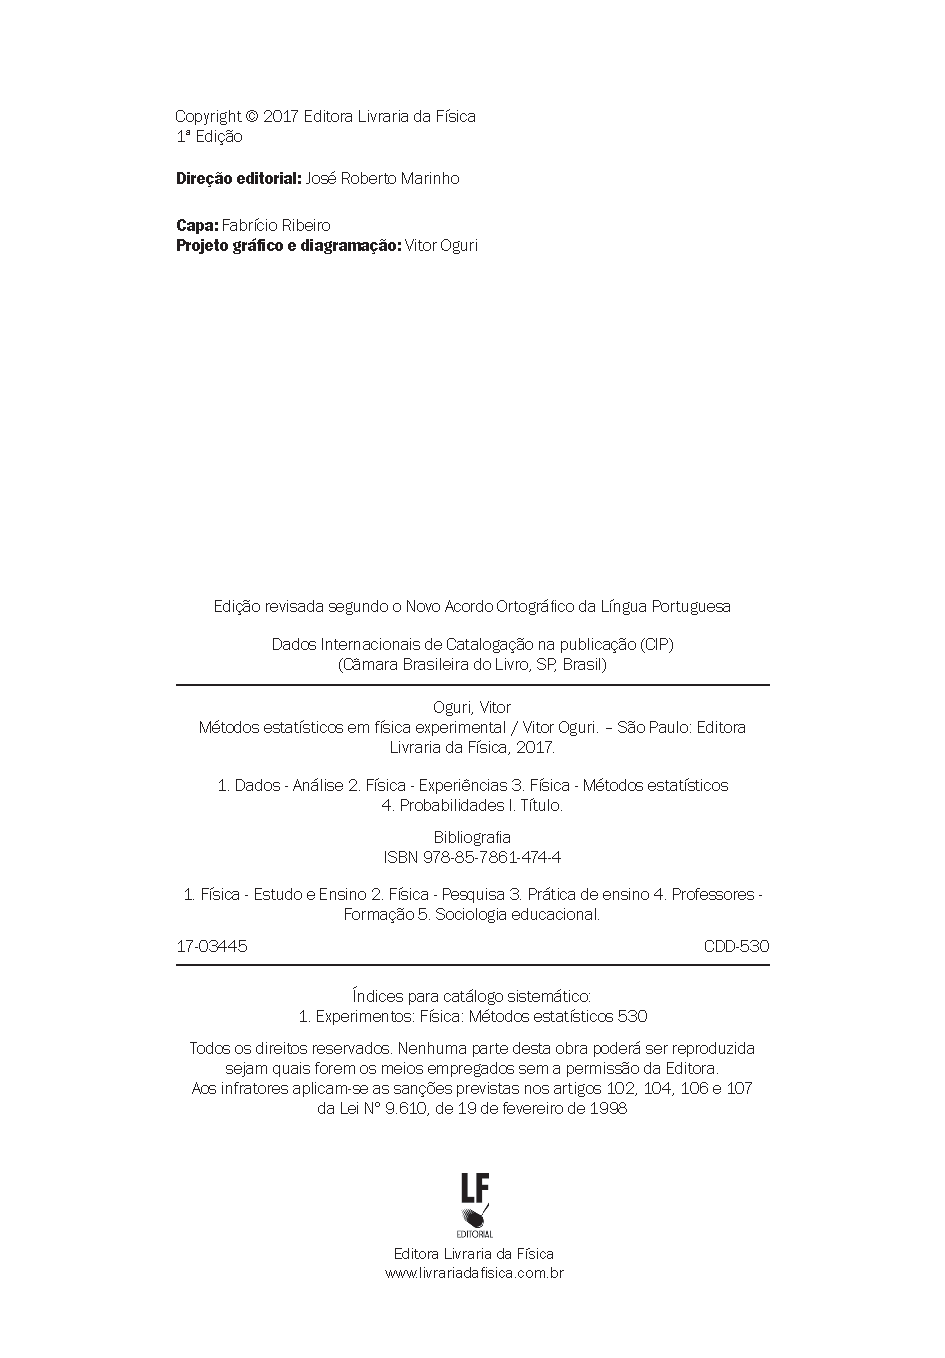
\includegraphics[height=23cm]{ficha_catalografica}}

\newpage

%\setcounter{page}{0}

\begin{flushright}
\begin{minipage}{3.cm}
\baselineskip=8pt
\hfill A Nobuo Oguri, \textit{in memoriam}

\end{minipage}
\end{flushright}

\vspace*{5.cm}
\begin{flushright}
\begin{minipage}{6.5cm}
\baselineskip=8pt
\textit{Se deseja saber a ess\^{e}ncia do m\'{e}todo cient\'{\i}fico, n\~{a}o preste aten\c{c}\~{a}o ao que lhe possa dizer um cientista. Observe o que ele faz.}
\medskip

\hfill {Albert Einstein}
\end{minipage}
\end{flushright}

%===============================================================
%\input{prefacio_oguri}
%\setcounter{chapter}{-1}
%\cleardoublepage%
%===============================================================
\chapter*{Pref\'{a}cio}
%===============================================================
%\ifpdf\relax\else
%\pagestyle{fancy}
%\fi
\addcontentsline{toc}{chapter}{Pref\'{a}cio}%
\markboth{Pref\'{a}cio}{Pref\'{a}cio}%

\baselineskip=14pt

\vspace*{-0.7cm}
\paragraph*{}
Este livro \'{e} fruto da experi\^{e}ncia do autor em an\'{a}lise de dados em experimentos de F\'{\i}sica, desde  sua forma\c{c}\~{a}o inicial nos anos de 1980, na \'{a}rea de raios X e radia\c{c}\~{a}o s\'{\i}ncrotron, nos laborat\'{o}rios  da faculdade de engenharia f\'{\i}sica da Universidade de T\'{o}quio e na {\it Photon Factory} do KEK,\footnote{Acelerador  S\'{\i}ncrotron do  Laborat\'{o}rio de Altas Energias do Jap\~{a}o, em Tsukuba.} at\'{e} a sua participa\c{c}\~{a}o em  grandes experimentos de Altas Energias; DZero  do Fermilab\footnote{Fermi National Accelerator Laboratory, Batavia, Illinois, USA.}  e CMS do CERN,\footnote{Centro Europeu de F\'{\i}sica de Part\'{\i}culas, Genebra, Su\'{\i}\c{c}a.} nos anos de 1991 at\'{e} 2013.

 O material selecionado \'{e} abordado no corpo do texto de modo intuitivo, es\-pe\-ran\-do-se que o leitor tenha familiaridade apenas com os t\'{o}picos b\'{a}sicos de um curso de C\'{a}lculo Diferencial e Integral,  e com alguns conceitos da Estat\'{\i}stica,  todos temas abordados regularmente nos ciclos b\'{a}sicos dos cursos de F\'{\i}sica, Qu\'{\i}mica  e Engenharias.

O texto que serviu de ponto de partida do livro corresponde \`{a}s notas de aula da disciplina de Tratamento estat\'{\i}stico de dados em F\'{\i}sica, mi\-nistrada pelo autor em diversos per\'{\i}odos, ao longo dos \'{u}ltimos 10 anos, na gradua\c{c}\~{a}o e no programa de p\'{o}s-gradua\c{c}\~{a}o do Instituto de F\'{\i}sica Armando Dias Tavares da  Universidade do Estado do Rio de Janeiro (Uerj).
	
Apesar de muitos exemplos serem tomados da \'{a}rea de Altas Energias, as ferramentas e os  m\'{e}todos estat\'{\i}sticos apresentados podem ser utilizados em qualquer experimento que envolva processos aleat\'{o}rios.

O autor agradece aos colegas do Departamento de F\'{\i}sica de Altas Energias da Uerj, Alberto Franco de S\'{a} Santoro, Francisco Caruso, Jos\'{e} Roberto Mahon e Dilson de Jesus Dami\~{a}o, pela leitura, cr\'{\i}ticas  e sugest\~{o}es ao texto.

Um agradecimento especial \`{a} Stella Maris Amadei pela cuidadosa  leitura de diferentes vers\~{o}es de todos os  cap\'{\i}tulos e pelas sugest\~{o}es de estilo.


\vspace*{0.2cm}

%\leftline{\textit{Rio de Janeiro}}

%\vspace*{0.3cm}
\rightline{\textbf{V.O.}}
%\clearpage
%\par
%\vfill

\newpage \ \\
\thispagestyle{empty}



%===============================================================
% \newpage
% \thispagestyle{empty}
% \ \\
%===============================================================
%\input{apresentacao}
%===============================================================

%\ifpdf\relax\else
\begin{flushleft}\protect
\tableofcontents\protect%
\end{flushleft}\protect

\vfill

%\newpage

\endinput
%===============================================================
%\markboth{ }{ }\thispagestyle{myheadings}
\clearpage

\newpage \ \\
\thispagestyle{empty}

\newpage

\pagenumbering{arabic}
\markboth{ }{ }
\pagestyle{fancy}
%\pagestyle{myheadings}
\parskip 2mm
%
\baselineskip=15pt


%\setcounter{chapter}{1}
%\setcounter{page}{10}
%\fancyhead[LE]{\thepage \quad  \footnotesize\rm\nouppercase{\sc Acaso e necessidade} }
%\fancyhead[LE]{\scriptsize\nouppercase{\sc\rightmark} \quad \footnotesize \rm\nouppercase{\sc  Cap\'{\i}tulo~\thechapter}}
\fancyhead[CE]{\scriptsize\nouppercase{\sc\rightmark}}
%\newpage
\thispagestyle{empty}

\markboth{ \mbox{ACASO E  NECESSIDADE} }{ \mbox{ACASO E NECESSIDADE} }

\noindent {\huge \bf 1 }

\vspace{1cm}
\noindent {\huge \bf Acaso e necessidade}

\addcontentsline{toc}{chapter}{1 \quad Acaso e necessidade}


\setcounter{chapter}{1}
\setcounter{equation}{0}

\label{Intro}

%\newpage
%\thispagestyle{empty}
%\chapter{A aleatoriedade dos fen\^{o}menos}
%\label{Intro}

%\pagenumbering{arabic}

\begin{flushright}
\begin{minipage}{6.5cm}
{\small
\baselineskip=8.5pt
{\it A incerteza \'{e} inevit\'{a}vel no c\'{a}lculo de resultados obser\-va\-cio\-nais. Em geral,  a teoria nos permite calcular somente a probabilidade de obtermos um resultado particular.}

\smallskip
\hfill P.~A.~M.~Dirac
}
\end{minipage}
\end{flushright}



\section{Aleatoriedade dos fen\^{o}menos} \index{fen\^{o}menos aleat\'{o}rios} \index{aleatoriedade dos fen\^{o}menos}

\paragraph*{}
Os fen\^{o}menos naturais podem ser classificados, quanto a possibilidade de ocorr\^{e}ncia, como determin\'{\i}sticos ou aleat\'{o}rios. Se os efeitos associados  a um fen\^{o}meno, devido a determinadas influ\^{e}ncias,  s\~{a}o inequivocamente previs\'{\i}veis, diz-se que os processos envolvidos s\~{a}o determin\'{\i}sticos. Por outro lado, se os efeitos associados a um fen\^{o}meno n\~{a}o s\~{a}o exatamente previs\'{\i}veis,
%mas podem ser associados a certas expectativas relativas de ocorr\^{e}ncia,
os processos envolvidos s\~{a}o ditos aleat\'{o}rios.

Segundo a vis\~{a}o cl\'{a}ssica da Ci\^{e}ncia, a n\~{a}o previsibilidade dos efeitos associados a um fen\^{o}meno estava associada a processos complexos que envolviam a intera\c{c}\~{a}o de um grande n\'{u}mero de sistemas simples.
Assim, o conceito de aleatoriedade estaria vinculado ao comportamento coletivo das mol\'{e}culas de um g\'{a}s, ou \`{a} enorme quantidade de n\'{u}cleos que participam do fen\^{o}meno da radioatividade.

Uma vez que a teoria fundamental da F\'{\i}sica Cl\'{a}ssica -- a Mec\^{a}nica de Newton -- descreve a evolu\c{c}\~{a}o temporal
  de um sistema composto de  part\'{\i}culas por equa\c{c}\~{o}es diferenciais ordin\'{a}rias, pressupunha-se que seu comportamento seria completamente determinado por sua condi\c{c}\~{a}o  inicial.\footnote{Caracterizada pelas posi\c{c}\~{o}es e velocidades iniciais de suas part\'{\i}culas constituintes.}  A aleatoriedade e o acaso em um fen\^{o}meno, ou em um experimento, eram atribu\'{\i}dos \`{a} incapacidade do observador em determinar as condi\c{c}\~{o}es iniciais, ou \`{a} complexidade dos arranjos experimentais.

  Em princ\'{\i}pio,  uma teoria fundamental deveria ser determin\'{\i}stica, tal que  uma dada condi\c{c}\~{a}o inicial estaria associada a um \'{u}nico resultado para a evolu\c{c}\~{a}o de um sistema f\'{\i}sico.
  Assim, teorias probabil\'{\i}sticas n\~{a}o seriam fundamentais, uma vez que poderiam admitir v\'{a}rios poss\'{\i}veis resultados para a evolu\c{c}\~{a}o de um sistema, ao associar expectativas distintas a cada um desses poss\'{\i}veis resultados.\footnote{Sabe-se hoje que, mesmo para sistemas com um pequeno n\'{u}mero de part\'{\i}culas, descritos por teorias causais, as quais em princ\'{\i}pio seriam determin\'{\i}sticas, pequenas perturba\c{c}\~{o}es iniciais podem dar origem a fen\^{o}menos ca\'{o}ticos n\~{a}o previs\'{\i}veis.}

%\pagebreak
Essa vis\~{a}o dos fen\^{o}menos, h\'{a} mil\^{e}nios arraigada no homem, foi tamb\'{e}m com\-par\-ti\-lha\-da por grandes expoentes do pensamento ocidental:

\begin{center}
\begin{minipage}{10cm}
 ``Nada acontece aleatoriamente; tudo acontece por al\-gu\-ma raz\~{a}o e por necessidade.''

\smallskip
\hfill Leucipo
\end{minipage}
\end{center}


\begin{center}
\begin{minipage}{10cm}
 ``Todos os eventos, mesmo aqueles que por sua ir\-re\-le\-v\^{a}n\-cia parecem n\~{a}o se relacionar \`{a}s grandes leis da natureza, delas constituem uma s\'{e}rie t\~{a}o necess\'{a}ria quanto as revolu\c{c}\~{o}es do Sol.''

\smallskip
\hfill P. S. Laplace
\end{minipage}
\end{center}

\begin{center}
\begin{minipage}{10cm}
 ``Deus n\~{a}o joga dados com o Universo.''

\smallskip
\hfill A. Einstein
\end{minipage}
\end{center}





Com o surgimento da Mec\^{a}nica Qu\^{a}ntica, em 1925, a aleatoriedade passa a ser considerada uma caracter\'{\i}stica intr\'{\i}nseca da evolu\c{c}\~{a}o dos fen\^{o}menos e sistemas f\'{\i}sicos, mesmo aqueles com poucos graus de liberdade.\footnote{Sistemas com um pequeno n\'{u}mero de part\'{\i}culas.}  A Mec\^{a}nica Qu\^{a}ntica estabelece que para cada problema h\'{a} de se calcular uma distribui\c{c}\~{a}o de probabilidades que conter\'{a} as informa\c{c}\~{o}es necess\'{a}rias \`{a} descri\c{c}\~{a}o do fen\^{o}meno estudado.

Segundo a Mec\^{a}nica Qu\^{a}ntica\cite{DIRAC}, os valores\footnote{Os valores de uma grandeza resultantes de um procedimento experimental (medi\c{c}\~{a}o) s\~{a}o denominados {\bf medidas}.} ou medidas poss\'{\i}veis de uma  grandeza f\'{\i}sica est\~{a}o associados a certas distribui\coes\ de probabilidade de ocorr\^encia.\footnote{Al\'{e}m do aspecto como expectativa de ocorr\^{e}ncia, o conceito de probabilidade admite outras interpreta\c{c}\~{o}es que ser\~{a}o apresentadas no Cap.~2.}

 Ainda que as medidas as\-so\-ci\-a\-das a uma grandeza n\~{a}o sejam inteiramente previs\'{\i}veis quando efetuadas sob as mesmas condi\c{c}\~{o}es experimentais,  essas medidas est\~{a}o  restritas a um conjunto de valores  condicionado pelas leis da F\'{\i}sica.
 %Nesse sentido, a aleatoriedade dos fen\^{o}menos significa uma  imprevisibilidade parcial.


De modo geral,  uma teoria probabil\'{\i}stica para o estudo dos fen\^omenos naturais ou dos sistemas f\'{\i}sicos deve prover regras que permitam determinar:
\begin{itemize}
\vspace{-0.2cm}
\item os valores (medidas) poss\'{\i}veis para as  grandezas associadas ao  fen\^omeno ou ao sistema  f\'{\i}sico;
\vspace{-0.2cm}
\item as respectivas pro\-ba\-bi\-li\-da\-des de ocorr\^encia das medidas das  grandezas, ou a distribui\cao\ dessas pro\-ba\-bi\-li\-da\-des.
\end{itemize}


\newpage \ \\
\thispagestyle{empty}

%\newpage
%\vspace*{0.5cm}




\markboth{ }{ }\thispagestyle{myheadings}

%\fancyhead[LE]{\thepage \quad  \footnotesize\rm\nouppercase{\sc M\'{e}todo da m\'{a}xima verossimilhan\c{c}a} }
\newpage
\thispagestyle{empty}

%\markboth{ \mbox{M\'{E}TODO  DA M\'{A}XIMA VEROSSIMILHAN\c{C}A} }{ \mbox{ESTIMADORES DE M\'{A}XIMA VEROSSIMILHAN\c{C}A} }

\noindent {\huge \bf 5 }

\vspace{1cm}
%\hspace*{-0.5cm} {\huge \bf M\'{e}todo~da~m\'{a}xima~verossimilhan\c{c}a} \index{metodo@m\'{e}todo! da m\'{a}xima verossimilhan\c{c}a}\index{maxima@m\'{a}xima verossimilhan\c{c}a! m\'{e}todo da}
\hspace*{-0.5cm} {\huge \bf Determina\c{c}\~{a}o de par\^{a}metros} \index{determina\c{c}\~{a}o de par\^{a}metros}\index{par\^{a}metros! determina\c{c}\~{a}o de}

%\addcontentsline{toc}{chapter}{5 \quad M\'{e}todo da m\'{a}xima verossimilhan\c{c}a}
\addcontentsline{toc}{chapter}{5 \quad Determina\c{c}\~{a}o de par\^{a}metros}
%ve\-ros\-si\-mi\-lhan\-\c{c}a

\setcounter{chapter}{5}
\setcounter{section}{0}
\setcounter{figure}{0}
\setcounter{table}{0}
\setcounter{equation}{0}
\label{Likeli}
%\newpage
%\thispagestyle{empty}

% \chapter{Estimativas de par\^{a}metros} \index{estimativas! de par\^{a}metros}
% \index{par\^{a}metros! estimativas de}
%\label{Erros}


%\def\figurename{\small Fig.~\ref{Erros}.}
%\def\tablename{\small Tab.~\ref{Erros}.}
%\newpage
%\ \\


\begin{flushright}
\begin{minipage}{8cm}
{\small
\baselineskip=8.5pt
{\it   Os problemas de estima\c{c}\~{a}o surgem quando conhecemos, ou consideramos que conhecemos, a forma da distribui\c{c}\~{a}o de frequ\^{e}ncias de uma popula\c{c}\~{a}o como uma fun\c{c}\~{a}o de um ou mais par\^{a}metros desconhecidos e,  a partir de uma amostra de dados, desejamos estimar os valores desses par\^{a}metros.}

\smallskip
\hfill R.~A.~Fisher
}
\end{minipage}
\end{flushright}





%\vspace{-0.1cm}
\section{Origens dos  m\'{e}todos estat\'{\i}sticos}\label{Erros}

%\vspace{-0.1cm}
\paragraph*{}
\ As origens dos m\'{e}todos e testes estat\'{\i}sticos modernos remontam aos trabalhos dos brit\^{a}nicos  Francis Galton  (1822-1911), \index{Pearson! Karl}Karl Pearson (1857-1936), \index{Gosset! William}William Gosset (1876-1937), \index{Fisher! Ronald}Ronald Fisher (1890-1962)  e do polon\^{e}s \index{Neyman! Jerzy}Jerzy Neyman (1894-1981).

Em sua obra cl\'{a}ssica, {\it The grammar of science},\footnote{Reimpresso  por   Dover Publications, Inc., em  2004.} em 1892,  Pearson estabelece  os modelos estat\'{\i}sticos como alternativa \`{a} vis\~{a}o determin\'{\i}stica do s\'{e}culo XIX, com base nos seguintes princ\'{\i}pios:

%\vspace{-0.1cm}
\begin{itemize}
%\vspace{-0.2cm}
\item  todo experimento est\'{a} sujeito a efeitos imprevistos e n\~{a}o observ\'{a}veis;
%\vspace{-0.2cm}
\item  os resultados de um experimento obedecem a distribui\c{c}\~{o}es de probabilidades caracterizadas por  par\^{a}metros e propriedades como: valor esperado, vari\^{a}ncia, assimetria e curtose.
%\vspace{-0.2cm}
%\item   os observ\'{a}veis na ci\^{e}ncia s\~{a}o as distribui\c{c}\~{o}es estat\'{\i}sticas que descrevem as probabilidades associadas \`{a}s observa\c{c}\~{o}es.
%\item \small M\'{e}todo dos momentos e teste de $\chi^{\scriptscriptstyle 2}$  \ (1900)
\end{itemize}

Para Pearson, as distribui\c{c}\~{o}es limites de pro\-ba\-bi\-li\-da\-des des\-cre\-viam ver\-da\-dei\-ra\-men\-te a cole\c{c}\~{a}o de dados (medidas)  resultante de  um experimento e,  a partir de um grande n\'{u}mero de medi\c{c}\~{o}es, os par\^{a}metros da distribui\c{c}\~{a}o real das medidas ou dos dados dos experimentos poderiam ser determinados.

Por outro lado, Fisher, em  seus trabalhos, sintetizados nos textos {\it Statistical meth\-ods for research workers} (1925)   e {\it The design of experiments} (1935), \footnote{Ambos reimpressos por Oxford University Press, em  2003.}  considera que os dados constituem uma amostra aleat\'{o}ria de uma popula\c{c}\~{a}o hipot\'{e}tica e, a partir de um experimento, obt\^{e}m-se apenas os {\bf estimadores} dos par\^{a}metros da distribui\c{c}\~{a}o hipot\'{e}tica dos dados.

Ao contr\'{a}rio dos par\^{a}metros (hipot\'{e}ticos), os estimadores s\~{a}o aleat\'{o}rios e devem ser avaliados, tanto segundo as distribui\c{c}\~{o}es  limites de probabilidades, quanto aos seguintes crit\'{e}rios:

\vspace{-0.3cm}
\begin{itemize}
\item  {\bf consist\^{e}ncia} -- quanto maior o n\'{u}mero ($N$) de dados em uma  amostra, mais pr\'{o}ximo um estimador $\hat a$  deve estar do valor ($a$) do par\^{a}metro;
         $$\displaystyle  \lim_{N \to \infty} \hat a = a $$
\vspace{-0.3cm}
    \item {\bf efici\^{e}ncia} -- quanto menor a vari\^{a}ncia  associada,  mais eficiente \'{e} o estimador;
    $$ V(\hat a_1) < V(\hat a_2)  \ \  \Longrightarrow \ \ \hat a_1 \ \mbox{mais eficiente}$$
\vspace{-0.3cm}
      \item {\bf n\~{a}o-tendenciosidade} -- o valor esperado de um estimador $E(\hat a)$ deve ser igual ao  valor ($a$) do par\^{a}metro.
          $$ E(\hat a) = a$$
%\item  Graus de liberdade \ (1922) e Likelihood  \ (1925)
\end{itemize}

Para Pearson e  Fisher, ou para a escola cl\'{a}ssica,  os par\^{a}metros (mesmo que sejam hipot\'{e}ticos) s\~{a}o fixos e os estimadores, aleat\'{o}rios; para a escola  bayesiana, no entanto, tanto os par\^{a}metros como os estimadores s\~{a}o aleat\'{o}rios.\index{estimadores! de m\'{a}xima verossimilhan\c{c}a}\index{maxima@m\'{a}xima verossimilhan\c{c}a! estimadores de}



\vspace{-0.1cm}
\section{O m\'{e}todo da m\'{a}xima verossimilhan\c{c}a de Fisher}
%\index{Fisher! m\'{e}todo da m\'{a}xima verossimilhan\c{c}a de}
 \index{metodo@m\'{e}todo! da m\'{a}xima verossimilhan\c{c}a}\index{maxima@m\'{a}xima verossimilhan\c{c}a! metodo@m\'{e}todo da}
 \index{Fisher! metodo@m\'{e}todo da m\'{a}xima verossimilhan\c{c}a}
 \label{MAX}
%\index{estimadores! de m\'{a}xima verossimilhan\c{c}a}
\vspace{-0.1cm}
\paragraph*{}
Seja $p(x|\theta)$ a distribui\c{c}\~{a}o de probabilidades  para as medidas de uma gran\-de\-za $x$, em que
$\theta$ \'{e} o par\^{a}metro da distribui\c{c}\~{a}o. Para  uma amostra  $(x_1, x_2, \dots, x_N)$ de $N$ me\-di\-das independentes de $x$, a pro\-ba\-bi\-li\-da\-de associada a es\-sa se\-qu\^{e}n\-cia particular de medidas \'{e}  dada por
$$  \prod_{i=1}^{N} p(x_i|\theta)  $$

%

\vspace{-0.2cm}
Se apenas a forma funcional da distribui\c{c}\~{a}o de probabilidades \apriori\ for conhecida, isto \'{e}, o par\^{a}metro for desconhecido, a  fun\c{c}\~{a}o definida por
%
\begin{equation}
 \label{vero1}
\fbox{~$\displaystyle  {\cal L} (x_1, x_2,  \dots,  x_N; \theta)  = K \ \prod_{i=1}^{N} p(x_i|\theta)
$~}
 \end{equation}
sendo $K$ \'{e} uma constante arbitr\'{a}ria, denominada
\index{fun\c{c}\~{a}o! de verossimilhan\c{c}a}{\bf fun\c{c}\~{a}o de verossimilhan\c{c}a} \cite{Fisher},\footnote{{\it Likelihood function}}\index{likeli@{\it likelihood function}} quantifica o qu\~{a}o veross\'{\i}mil \'{e} qualquer hip\'{o}tese relativa ao valor do par\^{a}metro.

 Nesse sentido,  para uma dada amostra de dados,  se $\theta_A$ e $\theta_B$ representam dois  poss\'{\i}veis  estimadores para o par\^{a}metro, e
%
$$ {\cal L} (\theta_A)  > {\cal L} (\theta_B) $$
diz-se que $\theta_A$ \'{e} um estimador mais veross\'{\i}mil para o par\^{a}metro do que $\theta_B$.
%
%Como a determina\c{c}\~{a}o dos par\^{a}metros de uma distribui\c{c}\~{a}o determina a depend\^{e}ncia expl\'{\i}cita funcional da distribui\c{c}\~{a}o, o procedimento \'{e} usualmente chamado tamb\'{e}m de {\bf ajuste de fun\c{c}\~{o}es}.
%
%%%%%%%%%%%%%%%%%%%%%%%%%%%%%%%%%%%%%%%%%%%%%%%%%%%%%%%%%%%%%%%%%
%\pagebreak
%
\begin{center}
\fbox{
\begin{minipage}{11.5cm}
Tomando-se o exemplo da se\c{c}\~{a}o~\ref{ex_bayes}: da caixa contendo 10 bolas, entre  vermelhas e azuis, da qual \'e extra\'{\i}da uma amostra com reposi\c{c}\~{a}o de 3 bolas vermelhas e uma azul.

\vspace{0.2cm}
  Para se estimar a quantidade $x$ de bolas azuis contidas na caixa,   a fun\c{c}\~{a}o de verossimilhan\c{c}a ${\cal L} (x)$ correspondente \`{a}  amostra obtida ser\'a dada pela probabilidade binomial de que   em 4 tentativas ($N=4$) de extra\c{c}\~{a}o de  bolas azuis haja apenas um sucesso ($m=1$).
   $${\cal L} (x) \ \propto \  B (m=1|N=4; p=x/10)$$
ou seja,
   $$ {\cal L} (x)\ \propto\  \frac{x}{10} \left( 1 - \frac{x}{10} \right)^3 =
   \frac{x (10 -x)^3}{10000}  \quad  \Rightarrow \quad {\cal L} (x) = x(10-x)^3 $$


\vspace{0.2cm}
De acordo com  a Tab.~\ref{azul_vero}, representada na Fig.~\ref{azul_vero_fig}, que mostra os   valores de  ${\cal L} (x)$ para todos os poss\'{\i}veis valores de $x$,  e segundo, ainda, o princ\'{\i}pio de Fisher, o valor 3 \'{e} a melhor estimativa para a quantidade de bolas azuis.
\end{minipage}
}
\end{center}
%
\begin{table}[hbtp]
\caption{Fun\c{c}\~{a}o de verossimilhan\c{c}a para uma amostra de um  sucesso ($m=1$) em 4 tentativas ($N=4$) de extra\c{c}\~{a}o de bolas azuis de uma caixa contendo 10 bolas.}
\label{azul_vero}
\vspace{-0.3cm}
\begin{center} \small
\begin{tabular}{c|l} \hline
$~~~x~~~$ & $~~~{\cal L} (x) \quad $  \\ \hline
~~~0~~~ & ~~~0~~~ \\
~~~1~~~ & ~~~729~~~ \\
~~~2~~~ & ~~~1024~~~ \\
~~~3~~~ & ~~~1029~~~ \\
~~~4~~~ & ~~~864~~~ \\
~~~5~~~ & ~~~625~~~ \\
~~~6~~~ & ~~~384~~~ \\
~~~7~~~ & ~~~189~~~ \\
~~~8~~~ & ~~~64~~~ \\
~~~9~~~ & ~~~9~~~ \\
~~~10~~~ & ~~~0~~~ \\ \hline
\end{tabular}
\end{center}
\end{table}



\begin{figure}[htbp]
\centerline{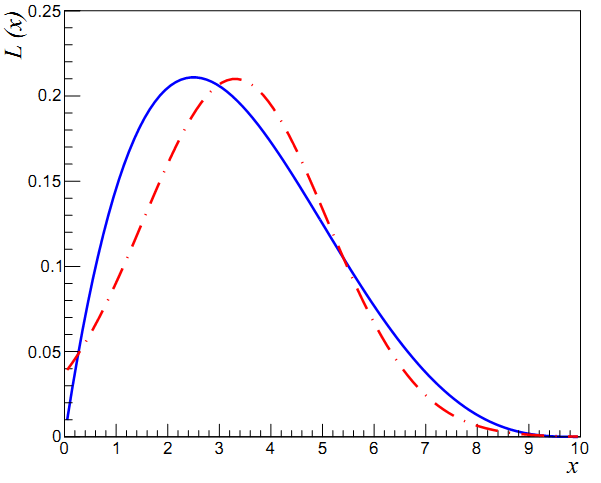
\includegraphics[width=7.cm]{veri_l1}}
\vspace{-0.2cm}
\caption{Fun\c{c}\~{a}o de verossimilhan\c{c}a (linha cont\'{\i}nua) para uma amostra de um sucesso em 4 tentativas  de extra\c{c}\~{a}o de bolas azuis de uma caixa contendo  10 bolas. A linha pontilhada \'{e} uma distribui\c{c}\~{a}o  gaussiana de mesmo valor esperado e desvio padr\~{a}o da fun\c{c}\~{a}o de verossimilhan\c{c}a normalizada.}
\label{azul_vero_fig}
\end{figure}


%

Ao se obter tr\^{e}s amostras  de quatro tentativas de extra\c{c}\~{a}o de bolas azuis, por exemplo, duas amostras de um sucesso ($m=1$) e uma de dois sucessos ($m=2$), a  fun\c{c}\~{a}o de verossimilhan\c ca \'e dada por (Fig.~\ref{verossimil})
   $${\cal L} (x) \ \propto \ B (1|4; x/10)^2 \times  B (2|4; x/10)$$
o que implica, igualmente, o valor 3 como a melhor estimativa para a quantidade de bolas azuis.
\begin{figure}[hbtp]
\centerline{\includegraphics[width=7.cm]{veri_l2}}
\vspace{-0.2cm}
\caption{Fun\c{c}\~{a}o de verossimilhan\c{c}a (linha cont\'{\i}nua)  para 2 amostras de um sucesso, e uma de dois sucessos em 4 tentativas de extra\c{c}\~{a}o  de bolas azuis de uma caixa contendo 10 bolas. A linha  pontilhada \'{e} uma gaussiana de mesmo valor esperado e desvio padr\~{a}o.}
\label{verossimil}
\end{figure}



%%%%%%%%%%%%%%%%%%%%%%%%%%%%%%%%%%%%%%%%%%%%%%%%%%%%%%%%%%%%%%%%%
%\pagebreak
Desse modo,  Fisher considera que o \index{estimadores! de m\'{a}xima verossimilhan\c{c}a}\index{maxima@m\'{a}xima verossimilhan\c{c}a! estimadores de}{\bf estimador  de m\'{a}xima verossimilhan\c{c}a}\footnote{Maximum likelihood estimator.} ($\hat \theta$)  para o  par\^{a}metro $\theta$ \'{e} aquele que maximiza a  fun\c{c}\~{a}o de verossimilhan\c{c}a, ou seja,
\begin{equation}
 \label{cond_vero}
\left. \frac{\partial {\cal L}}{\partial \theta}\right|_{\hat \theta} = 0
 \end{equation}

Uma vez que o logaritmo de ${\cal L}$ atinge seu m\'{a}ximo para o mesmo valor de $\theta$ e ${\cal L}$, a condi\c{c}\~{a}o de m\'{a}xima verossimilhan\c{c}a \'{e} expressa como
\begin{equation}
 \label{cond_vero2}
\left.  \frac{\partial \ln {\cal L}}{\partial \theta}\right|_{\hat \theta} = 0
 \end{equation}
ou seja, o estimador de m\'{a}xima verossimilhan\c{c}a \'{e} raiz da equa\c{c}\~{a}o anterior (Eq.~\ref{cond_vero2}).



%%%%%%%%%%%%%%%%%%%%%%%%%%%%%%%%%%%%%%%%%%%%%%%%%%%%%%%%%%%%%%%%%

%Para 30 amostras (Fig.~\ref{verossimil2}) de um sucesso (uma bola azul) e uma de dois sucessos (duas bolas azuis),obt\'{e}m-se
%   $${\cal L}^{31} (x) = B (1,4,x/10)^{30} \times  B (2,4,x/10)$$

%\begin{figure}[hbtp]
%\centerline{\includegraphics[width=8cm]{Fig/veri_l2}}
%\caption{Fun\c{c}\~{a}o de verossimilhan\c{c}a para 30 amostras de um sucesso, e uma de dois sucessos de extra\c{c}\~{a}o  e bolas azuis. A linha pontilhada \'{e} uma distribui\c{c}\~{a}o  gaussiana de mesma m\'edia e vari\^ancia.}
%\label{verossimil2}
%\end{figure}


\pagebreak
  Mesmo que o dom\'{\i}nio da vari\'{a}vel aleat\'{o}ria $x$ seja cont\'{\i}nuo, como usualmente as medidas de uma grandeza, as amostras constituem sequ\^{e}ncias discretas de valores organizados em $M$ classes de intervalos $\Delta_i$, como
$$ \Big\{ (x_1, x_2 = x_1 + \Delta_1) ;  (x_2, x_3 = x_2 + \Delta_2) ;  \dots  ; (x_M, x_{M+1} = x_M + \Delta_M) \Big\}$$


 Nesse caso, a probabilidade associada a essa sequ\^{e}ncia particular  \'{e}  dada por
%$$  \prod_{i=1}^{N} \int_{x_i}^{x_i + \Delta_i} \rho(x_i|\theta) \, \mbox{d}x_i $$
$$  \int_{x_1}^{x_2} \int_{x_2}^{x_3} \! \ldots  \int_{x_M}^{x_{M + 1}} \rho(x_1|\theta) \rho(x_2|\theta) \ldots \rho(x_M|\theta) \ \mbox{d}x_1 \, \mbox{d}x_2  \ldots \, \mbox{d}x_M $$

% Se os intervalos $\Delta_i$ s\~{a}o ``suficientemente pequenos'', pode-se escrever
%$$  \bigg( \underbrace{\prod_{j=1}^{N} \Delta_j}_{K = \, \mbox{\tiny cte.}} \bigg)  \prod_{i=1}^{N} \rho(x_i|\theta) $$
 e define-se a fun\c{c}\~{a}o de verossimilhan\c{c}a por
\begin{equation}
 \label{vero2}
\fbox{~$\displaystyle  {\cal L} (x_1, x_2, x_3 \dots  x_M; \theta)  = K \ \prod_{i=1}^{M} \rho(x_i|\theta)
$~}
 \end{equation}
em que $K$ \'{e} uma constante arbitr\'{a}ria.
\newpage
\section{Exerc\'{\i}cios}
\label{exerc_likeli}

\begin{itemize}

\item[\ref{exerc_likeli}.1)]
Ao colidir com a superf\'{\i}cie terrestre, um meteoro provoca uma cratera. A rela\c{c}\~{a}o esperada entre o di\^{a}metro ($D$) da cratera e a energia cin\'{e}tica ($E$) do meteoro no instante do impacto \'{e} dada por
$$ D = k E^{1/4} $$
em que $k$ \'{e} uma constante.

A tabela abaixo mostra os di\^{a}metros das depress\~{o}es causadas pelo impacto de diversas esferas de a\c{c}o sobre a areia contida em uma caixa, e as correspondentes  incertezas ($\epsilon_D$) e energias cin\'{e}ticas das esferas ao colidirem com a areia da caixa. As esferas s\~{a}o utilizadas para simularem a queda de meteoros.

\renewcommand{\arraystretch}{1.14}

%\vspace{0.1cm}

\hspace{0.3cm}
\begin{center}
{\small
\begin{tabular}{c|c|c}
        $E$(J)  &  $D$(cm)  &  $\epsilon_D$(cm) \\ \hline
     0,07 &   4,9 &  0,3  \\
     0,18 &   6,7 &  0,3  \\
     0,30 &    7,3 &   0,4  \\
     0,45  &   8,1  &  0,4   \\
     0,69 &    9,2 &   0,4  \\
  \hline
      \end{tabular}
}
\end{center}
\renewcommand{\arraystretch}{1}



\vspace{0.5cm}
A partir de um ajuste linear, determine uma estimativa para o expoente da rela\c{c}\~{a}o esperada entre a energia e o di\^{a}metro.

%\bibliographystyle{plainnat}
%\bibliography{biblio}


\end{itemize}

\markboth{ }{ }\thispagestyle{myheadings}

\fancyhead[LO]{\scriptsize\nouppercase{}}%
\fancyhead[RE]{\footnotesize\rm\nouppercase{\sc  Ap\^{e}ndice~\thechapter}}
%\fancyhead[RE]{\scriptsize\nouppercase{\sc\rightmark}}
%\newpage
\
\thispagestyle{empty}

\newpage
\
\thispagestyle{empty}

 \appendix

\markboth{ \mbox{AP\^{E}NDICE A} }{ \mbox{AP\^{E}NDICE A} }

%\noindent {\huge \bf Ap\^{e}ndices}
\

\vspace*{1.0cm}

\noindent {\huge \bf Ap\^{e}ndice A}

\label{topico}
\addcontentsline{toc}{chapter}{A \quad T\'{o}picos sobre probabilidades}


\setcounter{chapter}{1}

\setcounter{equation}{0}


\begin{flushright}
\begin{minipage}{6.5cm}
{\small
\baselineskip=8pt
{\it As loterias s\~{a}o formas de taxa\c{c}\~{a}o (aceitas livremente) das camadas menos privilegiadas da sociedade.}

\smallskip
\hfill D. Ruelle
}
\end{minipage}
\end{flushright}



%\newpage
%\thispagestyle{empty}

%\newpage
%\noindent
%{\bf Ap\^endices}
%\addcontentsline{toc}{section}{Ap\^endices}

% \appendix
% \chapter{T\'opicos sobre probabilidades}

%{\bf A \ \  T\'opicos sobre probabilidades}

%\addcontentsline{toc}{subsection}{I \ \  T\'opicos sobre probabilidades}


%\section{T\'opicos sobre probabilidades}
\label{topicos}

%\def\figurename{\small Fig.~\ref{topicos}.}
%\def\tablename{\small Tab.~\ref{topicos}.}

\section{Eventos equivalentes} \index{eventos! equivalentes}
%$\bullet$ {\bf Eventos equivalentes} :

\paragraph*{}
Se duas vari\'aveis aleat\'orias
$x$ e $y$ est\~ao relacionadas por $y=f(x)$  e $Y$ \'e um conjunto de
condi\coes\ (eventos) sobre a vari\'avel $y$~\footnote{Por exemplo,
uma rela\cao\ do tipo $y < a$, onde $a$ \'e uma constante.}
e $X = \{ x \ | \ f(x) \in Y \}$, diz-se que os conjuntos $X$ e $Y$ s\~ao
pro\-ba\-bi\-lis\-ti\-ca\-men\-te e\-qui\-va\-len\-tes, ou que
s\~ao eventos e\-qui\-va\-len\-tes, no sentido de que
suas probabilidades de ocorr\^encia s\~ao id\^enticas,

\vspace{.5cm}
\centerline{\fbox{\
$P(Y) = P(X)$ \ }}

\subsection*{$\bullet$ distribui\c{c}\~{o}es de probabilidades de eventos equivalentes}

\paragraph*{}
Sendo $f(x)$  a distribui\c{c}\~{a}o de probabilidades ({\bf pdf}) associada \`a vari\'avel $x$  e $y=h(x)$  uma outra vari\'avel aleat\'oria, por exemplo, $y=1+x=h(x)$ e $f(x) =x/2$ para $0 < x < 2$, a fun\cao\ de distribui\cao\  acumulada ({\bf fd})  \ $G(t)$ associada \`a $y$  ser\'a dada por
$$
\begin{array}{ll}
G(t) \! \! \! \! & =P(y\leq  t)  = P(1+x \leq t )  = P(x\leq t-1) \\
   \  \\
     &= \displaystyle \int_0^{t-1} f(x) \ {\rm d}x = \displaystyle \int_0^{t-1} \frac{x}{2} \ {\rm d}x
       = \frac{(t-1)^2}{4}
\end{array}
$$
\noindent e a pdf de $y$ por
$$g(y)= \frac{{\rm d}G}{{\rm d}y} = \frac{y-1}{2} $$

Como
$$ G(t) = P (x \leq \underbrace{t-1}_{h^{-1} (t)} ) =
F [ \underbrace{h^{-1} (t)}_{x(t)} ]$$
$$  \Downarrow $$
$$g(y) = \underbrace{\frac{{\rm d}F}{{\rm d}x}}_{f[x(y)]}
     \frac{{\rm d}(y)}{{\rm d}x}  = \frac{y-1}{2}$$

Admitindo que  $y=h(x)$ seja  uma fun\cao\ mon\'otona, de acordo com as propriedades,

\begin{itemize}
    \item[a)] $f$ crescente
    $$
\begin{array}{ll}
G(t)& =P(y\leq  t )  = P[ f(x)  \leq t ] \\
 & \\
     & = P [ (x\leq h^{-1} (t) ] = F [ h^{-1} (t) ]
\end{array}
$$
$$\Downarrow$$
$$\displaystyle  \underbrace{\frac{{\rm d}G}{{\rm d}y}}_{g(y)} =
  \underbrace{\frac{{\rm d}F}{{\rm d}x}}_{f(x)} \frac{{\rm d}x}{{\rm d}y}
  \ \ \ \ \left( \frac{{\rm d}x}{{\rm d}y} > 0 \right) $$

    \item[b)] $f$ decrescente
    $$
\begin{array}{ll}
G(t)& =P(y\leq t )  =  P [ (x > h^{-1} (t) ]  \\
  & \\
  & = 1 - P [ (x\leq h^{-1} (t) ]
\end{array}
$$
$$\Downarrow$$
$$ \begin{array}{ll}
\displaystyle  g(y) & = \displaystyle  - f(x) \ \frac{{\rm d}x}{{\rm d}y}
 \ \ \ \ \displaystyle  \left( \frac{{\rm d}x}{{\rm d}y} < 0 \right) \\
 & \\
   & \displaystyle  = f(x) \ \left| \frac{{\rm d}x}{{\rm d}y} \right|
   \end{array}
   $$
\end{itemize}

\noindent o   resultado  pode ser sistematizado como

\vspace{.5cm}
\centerline{\fbox{\ $ g(y) =  \displaystyle
f[x(y)] \ \left| \frac{{\rm d}x(y)}{{\rm d}y} \right| $ \ }}




\subsection*{$\bullet$ valor esperado  de fun\c{c}\~{a}o de uma   vari\'avel aleat\'oria}
\index{valor! esperado}
%\addcontentsline{toc}{section}{I Valor m\'edio de fun\cao\ de uma   vari\'avel aleat\'oria}

 \paragraph*{}
   A  determina\cao\  do valor esperado de uma fun\cao\  $y=h(x)$ de uma vari\'avel aleat\'oria $x$ cuja  pdf \'{e}  $f(x)$ \'{e} dada por $$ \langle y \rangle = \int_{-\infty}^{\infty} y \,  g(y) \ {\rm d}y$$
sendo $g(y)$ a pdf  de $y$.

No entanto, uma vez que
    $$
g(y)  = f[x(y)] \ \displaystyle \frac{{\rm d}x}{{\rm d}y} $$
$$   \Downarrow $$
$$
  \langle y \rangle  = \displaystyle
  \int_{-\infty}^{\infty} y \  f[x(y)] \
  \left| \frac{{\rm d}x}{{\rm d}y} \right|  \ {\rm d}y  = \displaystyle
  \int_{-\infty}^{\infty} y \  f[x(y)] \
   \frac{{\rm d}x}{{\rm d}y}  \ {\rm d}y
  $$

\noindent
\vspace{0.3cm}
o valor m\'{e}dio pode ser determinado pela {\bf pdf} de $x$,  por

\vspace{.2cm}
\centerline{\fbox{\ $    \langle h(x) \rangle  =  \displaystyle
  \int_{-\infty}^{\infty}  \  h(x) \
   f(x)   \ {\rm d}x  $ \ }}


\markboth{ }{ }\thispagestyle{myheadings}

%\pagestyle{fancy}
\fancyhead[CO]{}
\fancyhead[LO]{\scriptsize\nouppercase{\sc\rightmark}}%
\fancyhead[RO]{~\mbox{\thepage}\hspace{0.0em}}%
\fancyhead[CE]{}
\fancyhead[LE]{\thepage}
\fancyhead[RE]{\footnotesize\rm\nouppercase{\sc \rightmark}}

%\newpage
%\thispagestyle{empty}
%\
%################ ARTIGOS #################
%\smally}{90}
\begin{thebibliography}{90}


\bibitem{DIRAC} P.~A.~M.~Dirac,
    {\it The Principles of Quantum Mechanics},
    Oxford University Press, 1958.

\bibitem{Fisher} R.~A.~Fisher,
    {\it On the Mathematical Foundations of Theoretical Statistics},
    {\it Philosophical Transactions of the Royal Society},  v. 222, 309-368, 1922.

\bibitem{Fisher0} R.~A.~Fisher,
    {\it Applications of ``Student's'' Distribution}, Metron {\bf 5}, 90-104, 1925.

 \bibitem{STIGLER} S.~M.~Stigler,
    {\it The History of  Statistics: The Measurement of Uncertainty before 1900},
    Harvard University Press, 1986.

\bibitem{Student} Student,
    {\it The Probable Error of a Mean},
Biometrika,  Vol. VI (1908), 1-25, 1900.

\end{thebibliography}

\small

%\nocite{*}


{\small
%\input{fisgeral-F1-ind}
\clearpage\markboth{ \mbox{} }{ \mbox{} }

%\newpage
%\def\listfigurename{Figuras}
%\listoffigures

%\newpage
%\def\listtablename{Tabelas}
%\listoftables


\newpage
\markboth{\'{I}ndice remissivo}{\'{I}ndice remissivo}
\pagestyle{fancy}
\fancyhead[LO]{\scriptsize\nouppercase{\sc \'{I}ndice remissivo}}%
%\fancyhead[RO]{~\mbox{\thepage}\hspace{-1.5em}}%
\fancyhead[RO]{~\mbox{\thepage}\hspace{0.0em}}%
\fancyhead[LE]{\thepage}
\fancyhead[RE]{\footnotesize\rm\nouppercase{\sc \'{I}ndice remissivo}}

\def\indexname{\'{I}ndice remissivo}
\printindex %\thispagestyle{empty}
}



\end{document}



